\chapter{Exerimental Studies and Results}
\label{chapter4}

	The proposed two architectures described in the previous section has been tested upon four publicly available benchmark single fingerprint databases viz., (i) FVC2002(\ref{fig:figure4}), (ii) FVC2004 and (iii) FVC2006 (iv) IITD-MOLF and on IITK database which is not publicly available and the largest dataset comprising of more than 40, 000 images so far.
	
	The IITK dataset of single fingerprints consists of 41, 129 images collected using three different types of sensors viz., (i) Futronic (FS88H), (ii) Lumidigm V310 (V31X) and (iii) SecuGen Hamster I. All of them are of same 500 DIP, but the light source and the image size generated is different. All FVC dataset consists of images collected from four different types of sensors. We have trained the proposed model by taking only 10\% of the single finger print images as training set and rest 90\% as testing set, thus adopting a very difficult protocol.
	
	The results are computed for two different testing strategies namely (a) Intra sensor classification (b) Multi sensor classification. The Correct Classification Rate (CCR\%) is computed for performance evaluation, higher the value better is the result

\begin{figure}[htbp]
\centering
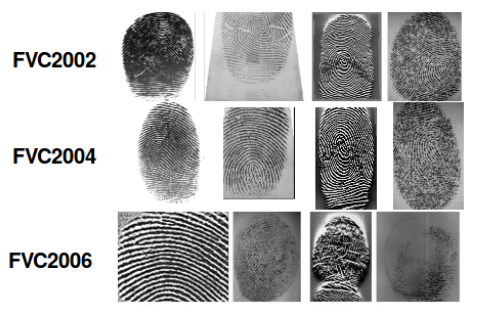
\includegraphics[scale=1]{./Chapter4/Figures/fvcsampleImages}
\caption{Sample FVC2002 dataset images}
\label{fig:figure5}
\end{figure}

\section{Intra-Model Classification}
		In this type of classification training and testing is performed on images acquired from same type of sensor model. Table~\ref{table3}, indicates the computed performance of two different proposed architectures on various datasets. The main phenomenon that we observed is that we are getting almost same type of CCR(\%) inspite of the fact of using two different kind of varied architectures. This can be attributed to the fact that fingerprint classification problem is a fine grain problem which does not require to learn features at the finest granular level and thus even shallow network is giving remarkable performance

\begin{longtable}[c]{|l|l|l|l|}
\caption{Intra Sensor qualitative performance in CCR(\%) on proposed architectures(DB1 means the images from the first sensor of the
corresponding dataset and same nomenclature is used for other
datasets)}
\label{table3}\\
\hline
Datasets & Sensor Type & Shallow & Deep \\ \hline
\endfirsthead
%
\endhead
%
FVC 2002 & \begin{tabular}[c]{@{}l@{}}DB1\\ DB2\\ DB3\\ DB4\\ Aggregate\end{tabular} & \begin{tabular}[c]{@{}l@{}}100\\ 99.17\\ 100\\ 99.72\\ 99.72\end{tabular} & \begin{tabular}[c]{@{}l@{}}100\\ 96.79\\ 99.72\\ 99.45\\ 98.99\end{tabular} \\ \hline
FVC 2004 & \begin{tabular}[c]{@{}l@{}}DB1\\ DB2\\ DB3\\ DB4\\ Aggregate\end{tabular} & \begin{tabular}[c]{@{}l@{}}100\\ 100\\ 99.85\\ 100\\ 99.96\end{tabular} & \begin{tabular}[c]{@{}l@{}}100\\ 100\\ 93.78\\ 99.17\\ 98.23\end{tabular} \\ \hline
FVC 2006 & \begin{tabular}[c]{@{}l@{}}DB1\\ DB2\\ DB3\\ DB4\\ Aggregate\end{tabular} & \begin{tabular}[c]{@{}l@{}}100\\ 100\\ 100\\ 99.93\\ 99.98\end{tabular} & \begin{tabular}[c]{@{}l@{}}99.87\\ 99.28\\ 99.80\\ 100\\ 99.73\end{tabular} \\ \hline
IITD-MOLF & \begin{tabular}[c]{@{}l@{}}DB1\\ DB2\\ DB3\\ Aggregate\end{tabular} & \begin{tabular}[c]{@{}l@{}}100\\ 100\\ 99.92\\ 99.97\end{tabular} & \begin{tabular}[c]{@{}l@{}}100\\ 100\\ 100\\ 100\end{tabular} \\ \hline
IITK Dataset & \begin{tabular}[c]{@{}l@{}}Futronic\\ Lumidigm\\ SecuGen\\ Aggregate\end{tabular} & \begin{tabular}[c]{@{}l@{}}99.45\\ 100\\ 100\\ 99.82\end{tabular} & \begin{tabular}[c]{@{}l@{}}99.34\\ 100\\ 100\\ 99.78\end{tabular} \\ \hline
\end{longtable}

\section{Multi-Model Classification}
		In multi-sensor classification, data is fused together from various fingerprint sensors. We did this purposefully in order to check the generalizability of our proposed architectures. We have merged data from all FVC datasets i.e. FVC2002, FVC 2004 and FVC 2006. The combined dataset consists of 13, 063 images resulting from 12 different sensors and trained our network with 12 output neurons. We have trained our proposed model on 1306 images and tested on remaining 11, 757 images (i.e. 10\% training and 90\% testing). Table~\ref{table4} indicates the computed performance in terms of CCR(\%). We have observed that the obtained results are quite remarkable which depicts the high gener alizability of our proposed architectures. In this case also shallow networks are learning discriminative features quite well

\begin{longtable}[c]{|l|l|l|l|}
\caption{Mutli-sensor qualitative performance in CCR(\%) on proposed architectures (here in xDBy: x stands for FVC dataset number and y stands for sensor type of the corresponding dataset)}
\label{table4}\\
\hline
Dataset & Sensor Type & Shallow & Deep \\ \hline
\endfirsthead
%
\endhead
%
FVC Combined & \begin{tabular}[c]{@{}l@{}}2DB1\\ 2DB2\\ 2DB3\\ 2DB4\\ 4DB1\\ 4DB2\\ 4DB3\\ 4DB4\\ 6DB1\\ 6DB2\\ 6DB3\\ 6DB4\\ Aggregate\end{tabular} & \begin{tabular}[c]{@{}l@{}}98.75\\ 97.63\\ 100\\ 99.58\\ 99.31\\ 100\\ 100\\ 100\\ 100\\ 100\\ 99.86\\ 99.80\\ 99.58\end{tabular} & \begin{tabular}[c]{@{}l@{}}99.29\\ 98.37\\ 99.57\\ 99.72\\ 99.16\\ 100\\ 99.40\\ 97.47\\ 100\\ 100\\ 98.56\\ 100\\ 99.29\end{tabular} \\ \hline
\end{longtable}

\section{Robustness or Generalization Analysis}
In order to gain further insights in understanding the effectiveness and generalization of the proposed architecture we introduce some artifacts in the original image in the form of random-noise, rotation and occlusion. All these artifacts are done on a small validation-set comprising of 100 images for each sensor corresponding to IITK single fingerprint dataset.

\subsection{Rotation}

	In order to check the robustness of the proposed architecture the input fingerprint images have been rotated with different angles and the computed CCR\% is shown in Table~\ref{table5}. It can be inferred from Table~\ref{table5} as we increase the angle of rotation the performance of SecuGen sensor decreases drastically this can be attributed to the non uniformity of the image captured through it as clearly visible from Fig~\ref{fig:figure2}

\begin{longtable}[c]{|l|l|l|l|}
\caption{Rotation qualitative performance in CCR(\%) on validation set for shallow network architecture (here 2, 4, 6, 8 and 15 represents the angle of rotation in clockwise as well as in anti-clockwise direction )}
\label{table5}\\
\hline
Angle & Sensor                                                                & VGG                                                     & Resnet                                                   \\ \hline
\endfirsthead
%
\endhead
%
2     & \begin{tabular}[c]{@{}l@{}}Futronic\\ Lumidigm\\ SecuGen\end{tabular} & \begin{tabular}[c]{@{}l@{}}99\\ 100\\ 94.5\end{tabular} & \begin{tabular}[c]{@{}l@{}}100\\ 100\\ 100\end{tabular}  \\ \hline
4     & \begin{tabular}[c]{@{}l@{}}Futronic\\ Lumidigm\\ SecuGen\end{tabular} & \begin{tabular}[c]{@{}l@{}}99\\ 100\\ 84.5\end{tabular} & \begin{tabular}[c]{@{}l@{}}100\\ 100\\ 100\end{tabular}    \\ \hline
6     & \begin{tabular}[c]{@{}l@{}}Futronic\\ Lumidigm\\ SecuGen\end{tabular} & \begin{tabular}[c]{@{}l@{}}99\\ 100\\ 80\end{tabular}   & \begin{tabular}[c]{@{}l@{}}100\\ 100\\ 100\end{tabular}  \\ \hline
8     & \begin{tabular}[c]{@{}l@{}}Futronic\\ Lumidigm\\ SecuGen\end{tabular} & \begin{tabular}[c]{@{}l@{}}99\\ 100\\ 76\end{tabular}   & \begin{tabular}[c]{@{}l@{}}100\\ 100\\ 95.8\end{tabular} \\ \hline
\end{longtable}

\subsection{Occlusion}

	In order to test whether our proposed architecture is invariant to occlusion or not. We consider a patch of 90 X 90 in the input image and randomly occluded some percentage of pixels in it. The results in terms of CCR\% has been shown in Table~\ref{table6}. Surprisingly it can be inferred from Table~\ref{table6} that on increasing the occlusion in the image the performance of the network is not deteriorating. This abnormal behavior compel us to think what exactly our network is learning.

\begin{longtable}[c]{|l|l|l|l|}
\caption{Occlusion qualitative performance in CCR(\%) on validation set for shallow network architecture (here 1\%,5\% and 10\% are the percentage of pixels occluded in a region of 90 X 90 patch )
}
\label{table6}\\
\hline
Percentage & Sensor                                                                & VGG                                                       & Resnet                                                     \\ \hline
\endfirsthead
%
\endhead
%
1          & \begin{tabular}[c]{@{}l@{}}Futronic\\ Lumidigm\\ SecuGen\end{tabular} & \begin{tabular}[c]{@{}l@{}}100\\ 99.8\\ 99.8\end{tabular} & \begin{tabular}[c]{@{}l@{}}99.8\\ 100\\ 100\end{tabular}   \\ \hline
5          & \begin{tabular}[c]{@{}l@{}}Futronic\\ Lumidigm\\ SecuGen\end{tabular} & \begin{tabular}[c]{@{}l@{}}100\\ 99.6\\ 100\end{tabular}  & \begin{tabular}[c]{@{}l@{}}100\\ 100\\ 100\end{tabular}    \\ \hline
10         & \begin{tabular}[c]{@{}l@{}}Futronic\\ Lumidigm\\ SecuGen\end{tabular} & \begin{tabular}[c]{@{}l@{}}100\\ 99.2\\ 99.2\end{tabular} & \begin{tabular}[c]{@{}l@{}}99.4\\ 99.8\\ 98.6\end{tabular} \\ \hline
15         & \begin{tabular}[c]{@{}l@{}}Futronic\\ Lumidigm\\ SecuGen\end{tabular} & \begin{tabular}[c]{@{}l@{}}100\\ 98.2\\ 98.2\end{tabular} & \begin{tabular}[c]{@{}l@{}}99.6\\ 100\\ 98\end{tabular}    \\ \hline
\end{longtable}

		\subsection{Random Noise}

	In real life scenarios it is very difficult to get a perfect condition. Most of the time we end up with noise affecting our ideal conditions. In such cases it is essential that our architecture is robust for noise upto certain range. Table~\ref{table7} shows the result of adding random noise to our validation test data. It can be infered from Table~\ref{table7} that on increasing the random noise the performance of the Lumidigm sensor is decaying to a large extent. As it is clearly evident from Table~\ref{fig:figure2} that the Lumidigm sensor captured image is highly uniform in texture, so any small alteration or artifact in its texture greatly affects our network performance.

\begin{longtable}[c]{|l|l|l|l|}
\caption{ Random noise qualitative performance in CCR(\%) on validation set for shallow network architecture (here 0.01\%, 0.05\%, 0.1\% are the percentage of the random noise inserted in the input image of size 224 ∗ 224 )
}
\label{table7}\\
\hline
Percentage & Sensor                                                                & VGG                                                   & Resnet                                                   \\ \hline
\endfirsthead
%
\endhead
%
0.01       & \begin{tabular}[c]{@{}l@{}}Futronic\\ Lumidigm\\ SecuGen\end{tabular} & \begin{tabular}[c]{@{}l@{}}99\\ 100\\ 99\end{tabular} & \begin{tabular}[c]{@{}l@{}}100\\ 100\\ 100\end{tabular}  \\ \hline
0.05       & \begin{tabular}[c]{@{}l@{}}Futronic\\ Lumidigm\\ SecuGen\end{tabular} & \begin{tabular}[c]{@{}l@{}}99\\ 94\\ 98\end{tabular}  & \begin{tabular}[c]{@{}l@{}}100\\ 97.8\\ 100\end{tabular} \\ \hline
0.1        & \begin{tabular}[c]{@{}l@{}}Futronic\\ Lumidigm\\ SecuGen\end{tabular} & \begin{tabular}[c]{@{}l@{}}99\\ 50\\ 98\end{tabular}  & \begin{tabular}[c]{@{}l@{}}100\\ 85.6\\ 100\end{tabular} \\ \hline
\end{longtable}


\section{Layer Specific Feature Analysis}
	As it is clearly evident from Table~\ref{table7} that on increasing the amount of occlusion on our input images the performance of our proposed network is not degrading. This compels us to think some interesting questions: like what exactly our network is learning? Is there something wrong in its learning? Is there any kind of prestidigitation in our network? In order to answer these questions we try to visualize the feature maps learned by different layers of our proposed shallow network. For visualizing the feature-maps we took the SecuGen sensor of IIIT-K single fingerprint images. Part (a) of Fig~\ref{fig:figure4} shows the features learned by our proposed shallow network. It is clearly evident from the Fig~\ref{fig:figure4} , that initial convolutional layers are learning general specific features, while as we go deeper and deeper more sensor specific features, localized and sparse features are learned. It can be observed in Part (a) of Fig~\ref{fig:figure4} that layer 3 and layer 6 are trying to understand the textual patterns of the image, but as we move deeper in the network like in layer 9 and layer 14 more emphasis is given to learn the shape and the background of the image rather than its textual patterns. By observing this we realize that our network is smart enough instead of learning finer granular level discriminative information to distinguish between different sensors it learned the background and shape of the image instead of its textual features.

	This could be the main reason for the exceptionally high performance of the network in case of occluded images. In order to prove it we did another set of experimentation in this we crop an input image from the middle in the size of 90 X 90 patch and paste it over a white background. By doing this we have forcefully made the background of all the images same, in-order to force our network to learn textual features instead of background. It is clearly evident from Fig~\ref{fig:figure4} that now our network is learning textual patterns instead of background. It is also proved by the results that we obtained after adding occlusion on this set of images

\begin{figure}[htbp]
\centering
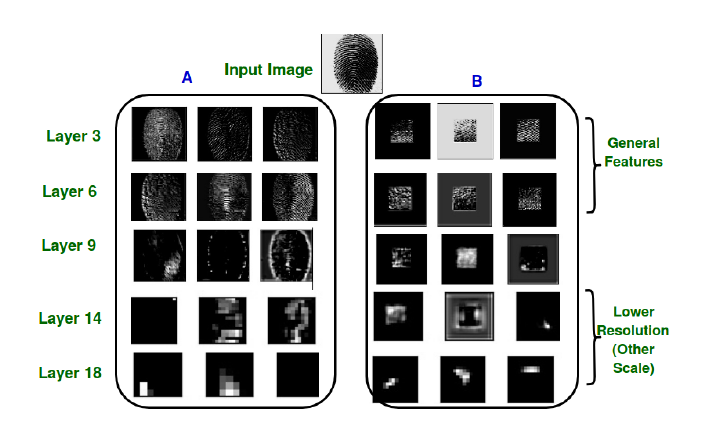
\includegraphics[scale=1]{./Chapter4/Figures/FeatureAnalysis}
\caption{Comparative Feature Analysis.}
\label{fig:figure4}
\end{figure}

\section{Training }
First of all VGG was used instead of CNN-F network in the hashing network. As we don't have too much data, we used pre-trained VGG16 model trained on imagenet weights, then to fine tune the model to our fingerprint data, we used IIT-K data consisting of images of 3 different sensors with a total of about 40,000 images in the dataset. To fine tune our model on this dataset, we opted for three different ways:-

\subsection {\bf Auto-Encoder:} 
Autoencoder are used for unsupervised learning in a neural network. We try to train our VGG model using autoencoder by simply applying a decoder at the end of the VGG model. An autoencoder tries to compress the data into a short code which our VGG was doing, then decodes the short code back to the original data, thus forcing our VGG model to learn deeper feature of our dataset. The first layer in encoder might try to encode easy features like shape and qualtiy of fingerprints, the second might analyze first layer's output and then encode less local features like various patterns in our fingerprints, minutiae etc and then finally forcing our model to encode the whole fingerprint image. After training our model we did two kind of experiment to check the efficiency of our model
\begin{figure}[htbp]
\centering
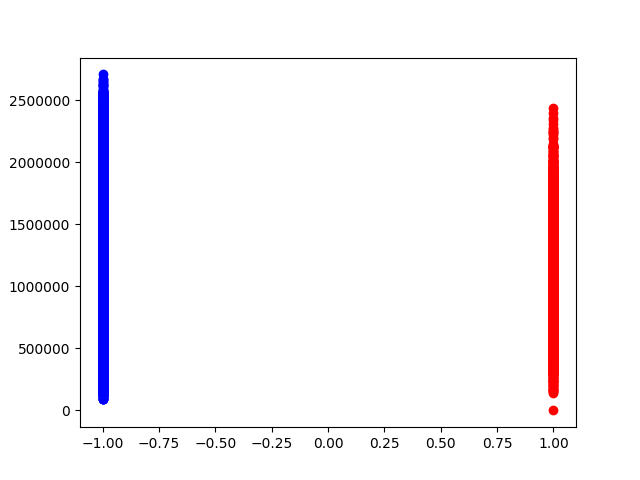
\includegraphics[scale=1]{./Chapter4/Figures/AE_norms_pos_neg}
\caption{L2 distance for all positive and negative pairs. Here X = 1 stands for positive and X = -1 stands for negative pairs. Y axis represents the value of L2 distance}
\label{fig:figure7}
\end{figure}
\begin{itemize}
    \item We took all the positive pairs (similar pairs) in our dataset and then calculated the final output of the last layer of our hashing model (DADH) and calculated the L2 distance between them, similarly we did for the all the negative pairs and plotted both of them as shown in \ref{fig:figure7}. But we can see that all the positive pairs and negative pairs lies closely instead of positive pairs tending towards zero and negative pairs tending away from zero. This states that our model is not properly trained with the help of autoencoder.
    \item Now we took different subjects and tried to plot them into tsne \cite{Maaten2008VisualizingDU} curve to see the separability between the different subjects. We predicted the output of different subjects and their similar images in group of 10 from our hashing model as shown in \ref{fig:figure8}
\begin{figure}[htbp]
\centering
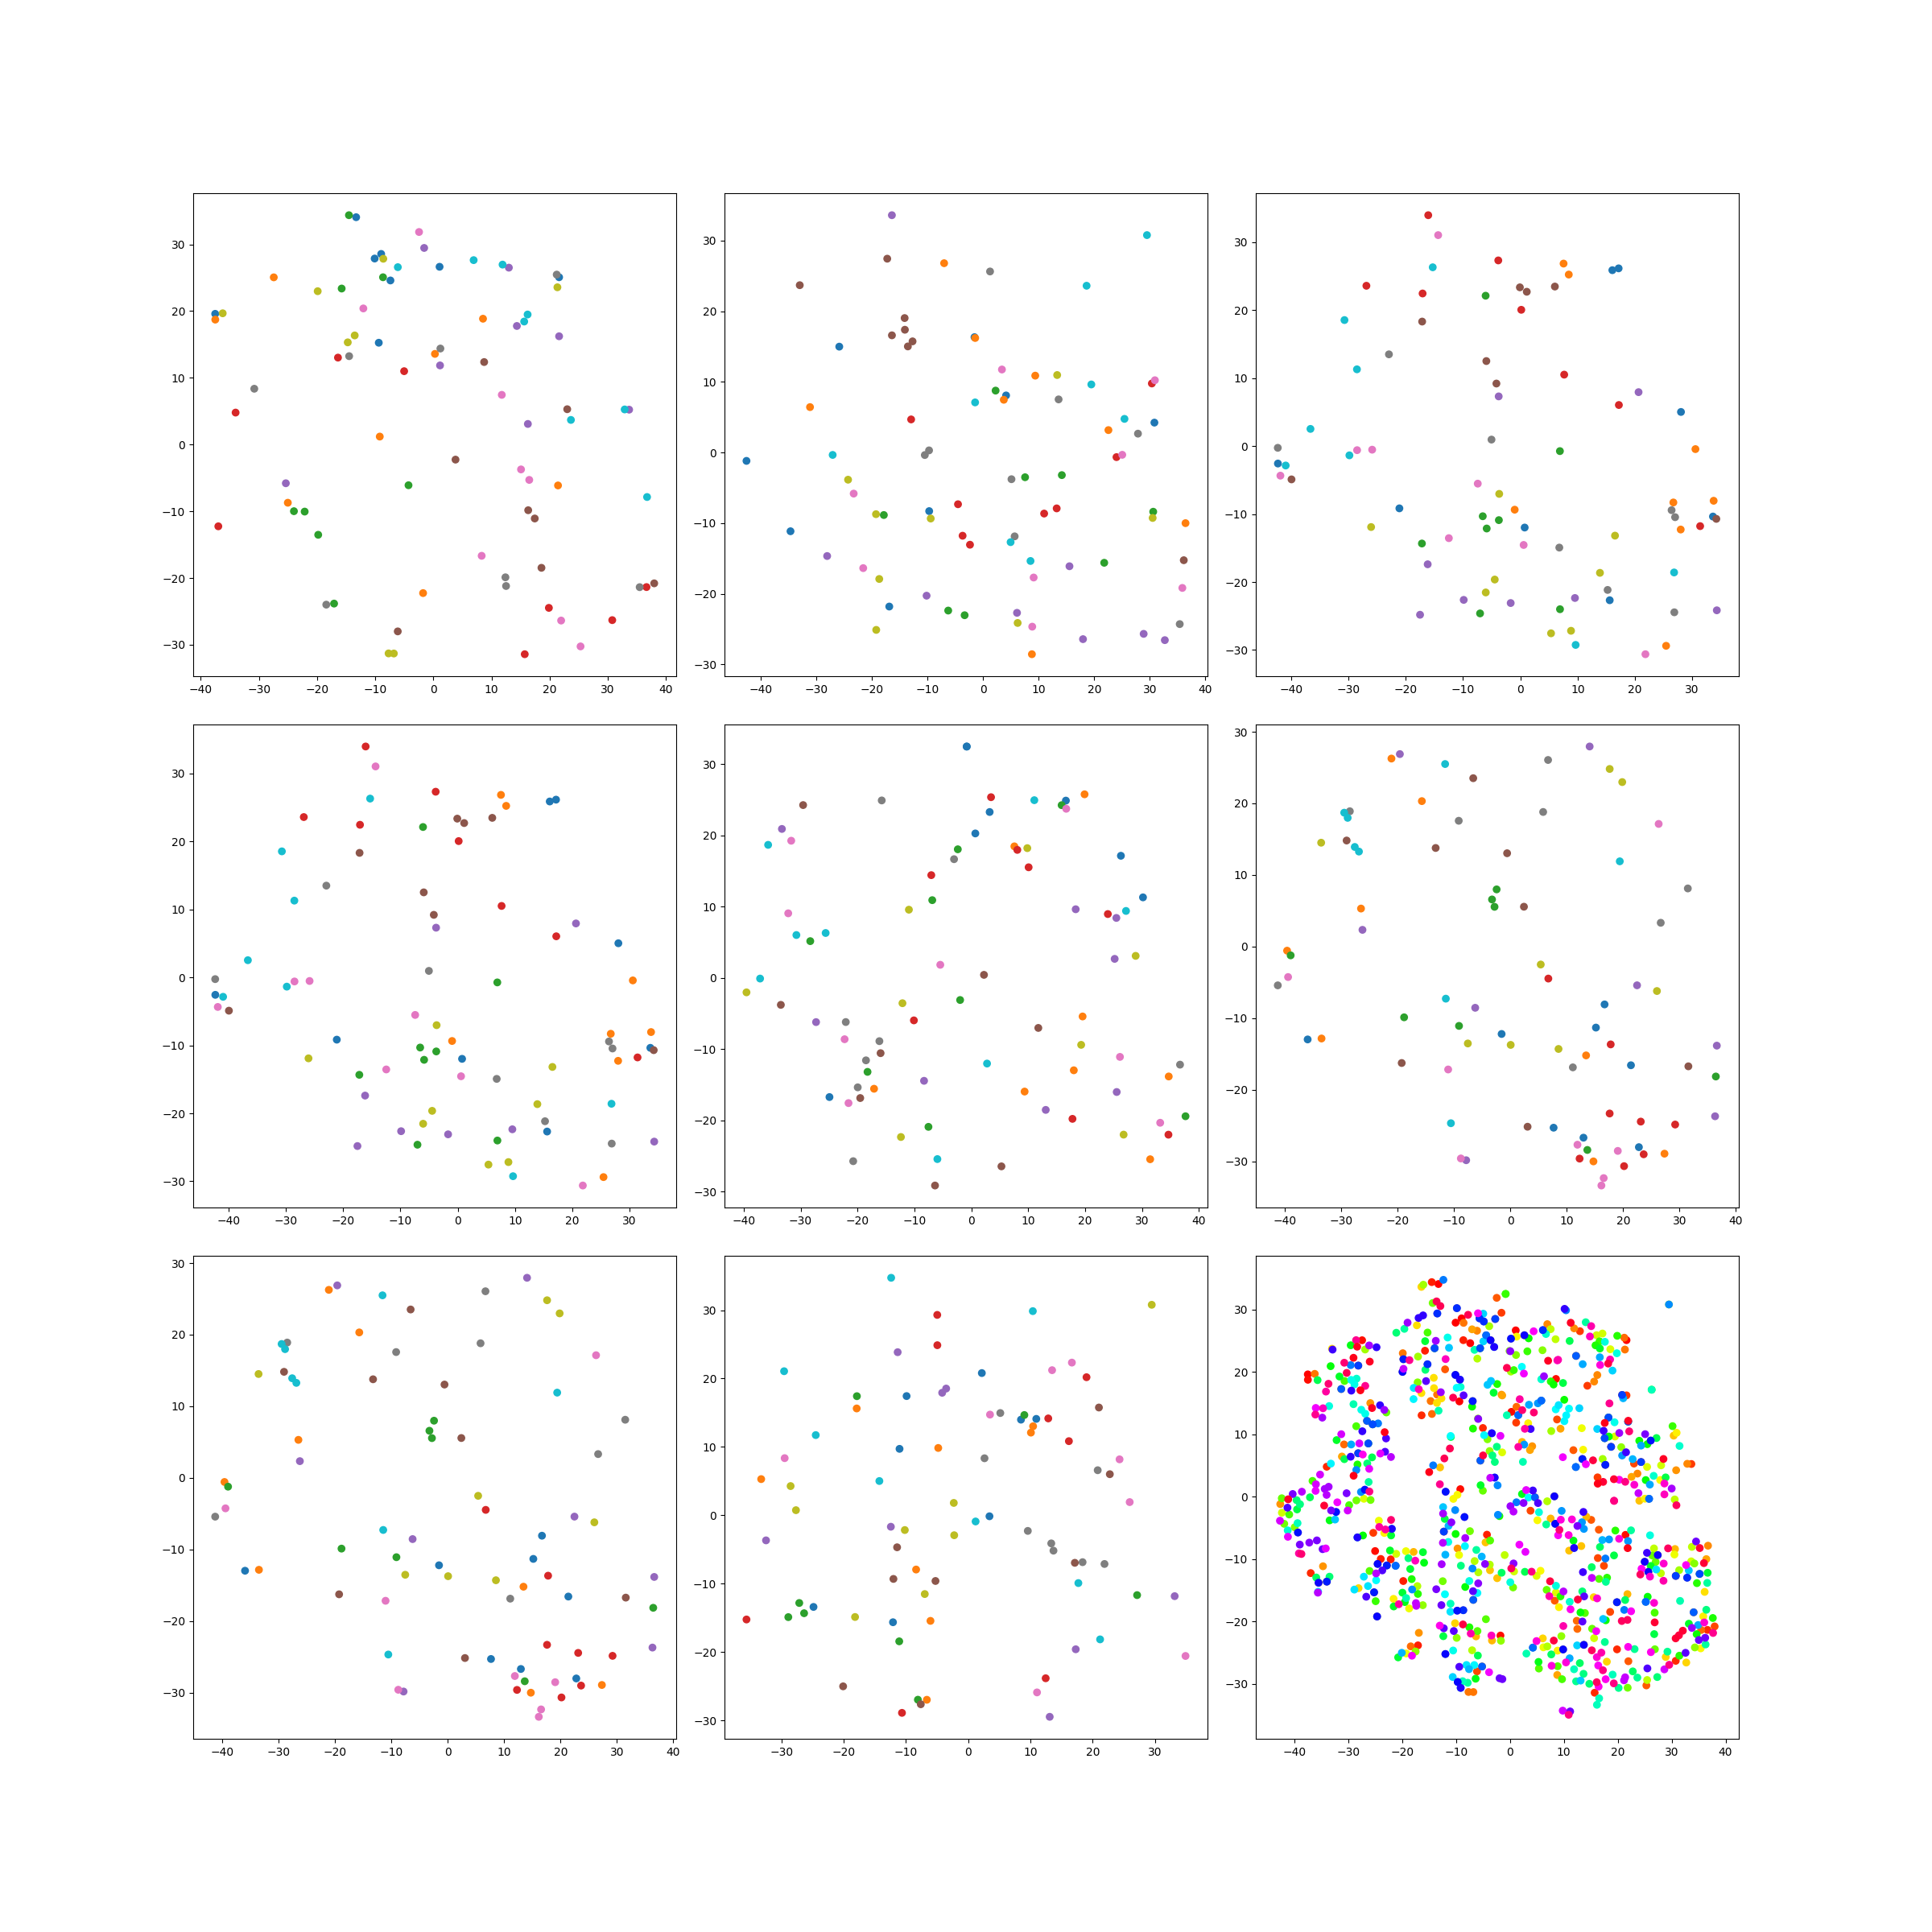
\includegraphics[scale=0.3]{./Chapter4/Figures/AEtsne_1}
\caption{First eight curve include graphs for 10 different subjects each, last curve shows separability of all 100 subjects.}
\label{fig:figure8}
\end{figure}
    \end{itemize}

\subsection{VGG as classifier}
Now we took this problem as a classification problem of 100 classes (FVC dataset contains 100 subjects per sensor), and we tried to plot the t-sne \cite{Maaten2008VisualizingDU} as well as the L2 distance between all the positive and negative pairs. We trained our VGG model on all the subjects with all the similar images as the images within same class. The plot to L2 distance and t-sne \cite{Maaten2008VisualizingDU} are shown as \ref{fig:figure9} and \ref{fig:figure10} respectively.

\begin{figure}[htbp]
\centering
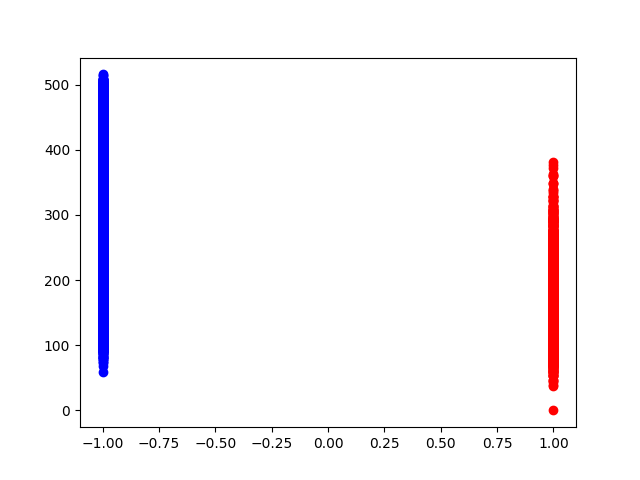
\includegraphics[scale=1]{./Chapter4/Figures/CLSnorms_pos_neg_1}
\caption{L2 distance for all positive and negative pairs. Here X = 1 stands for positive and X = -1 stands for negative pairs. Y axis represents the value of L2 distance}
\label{fig:figure9}
\end{figure}

\begin{figure}[htbp]
\centering
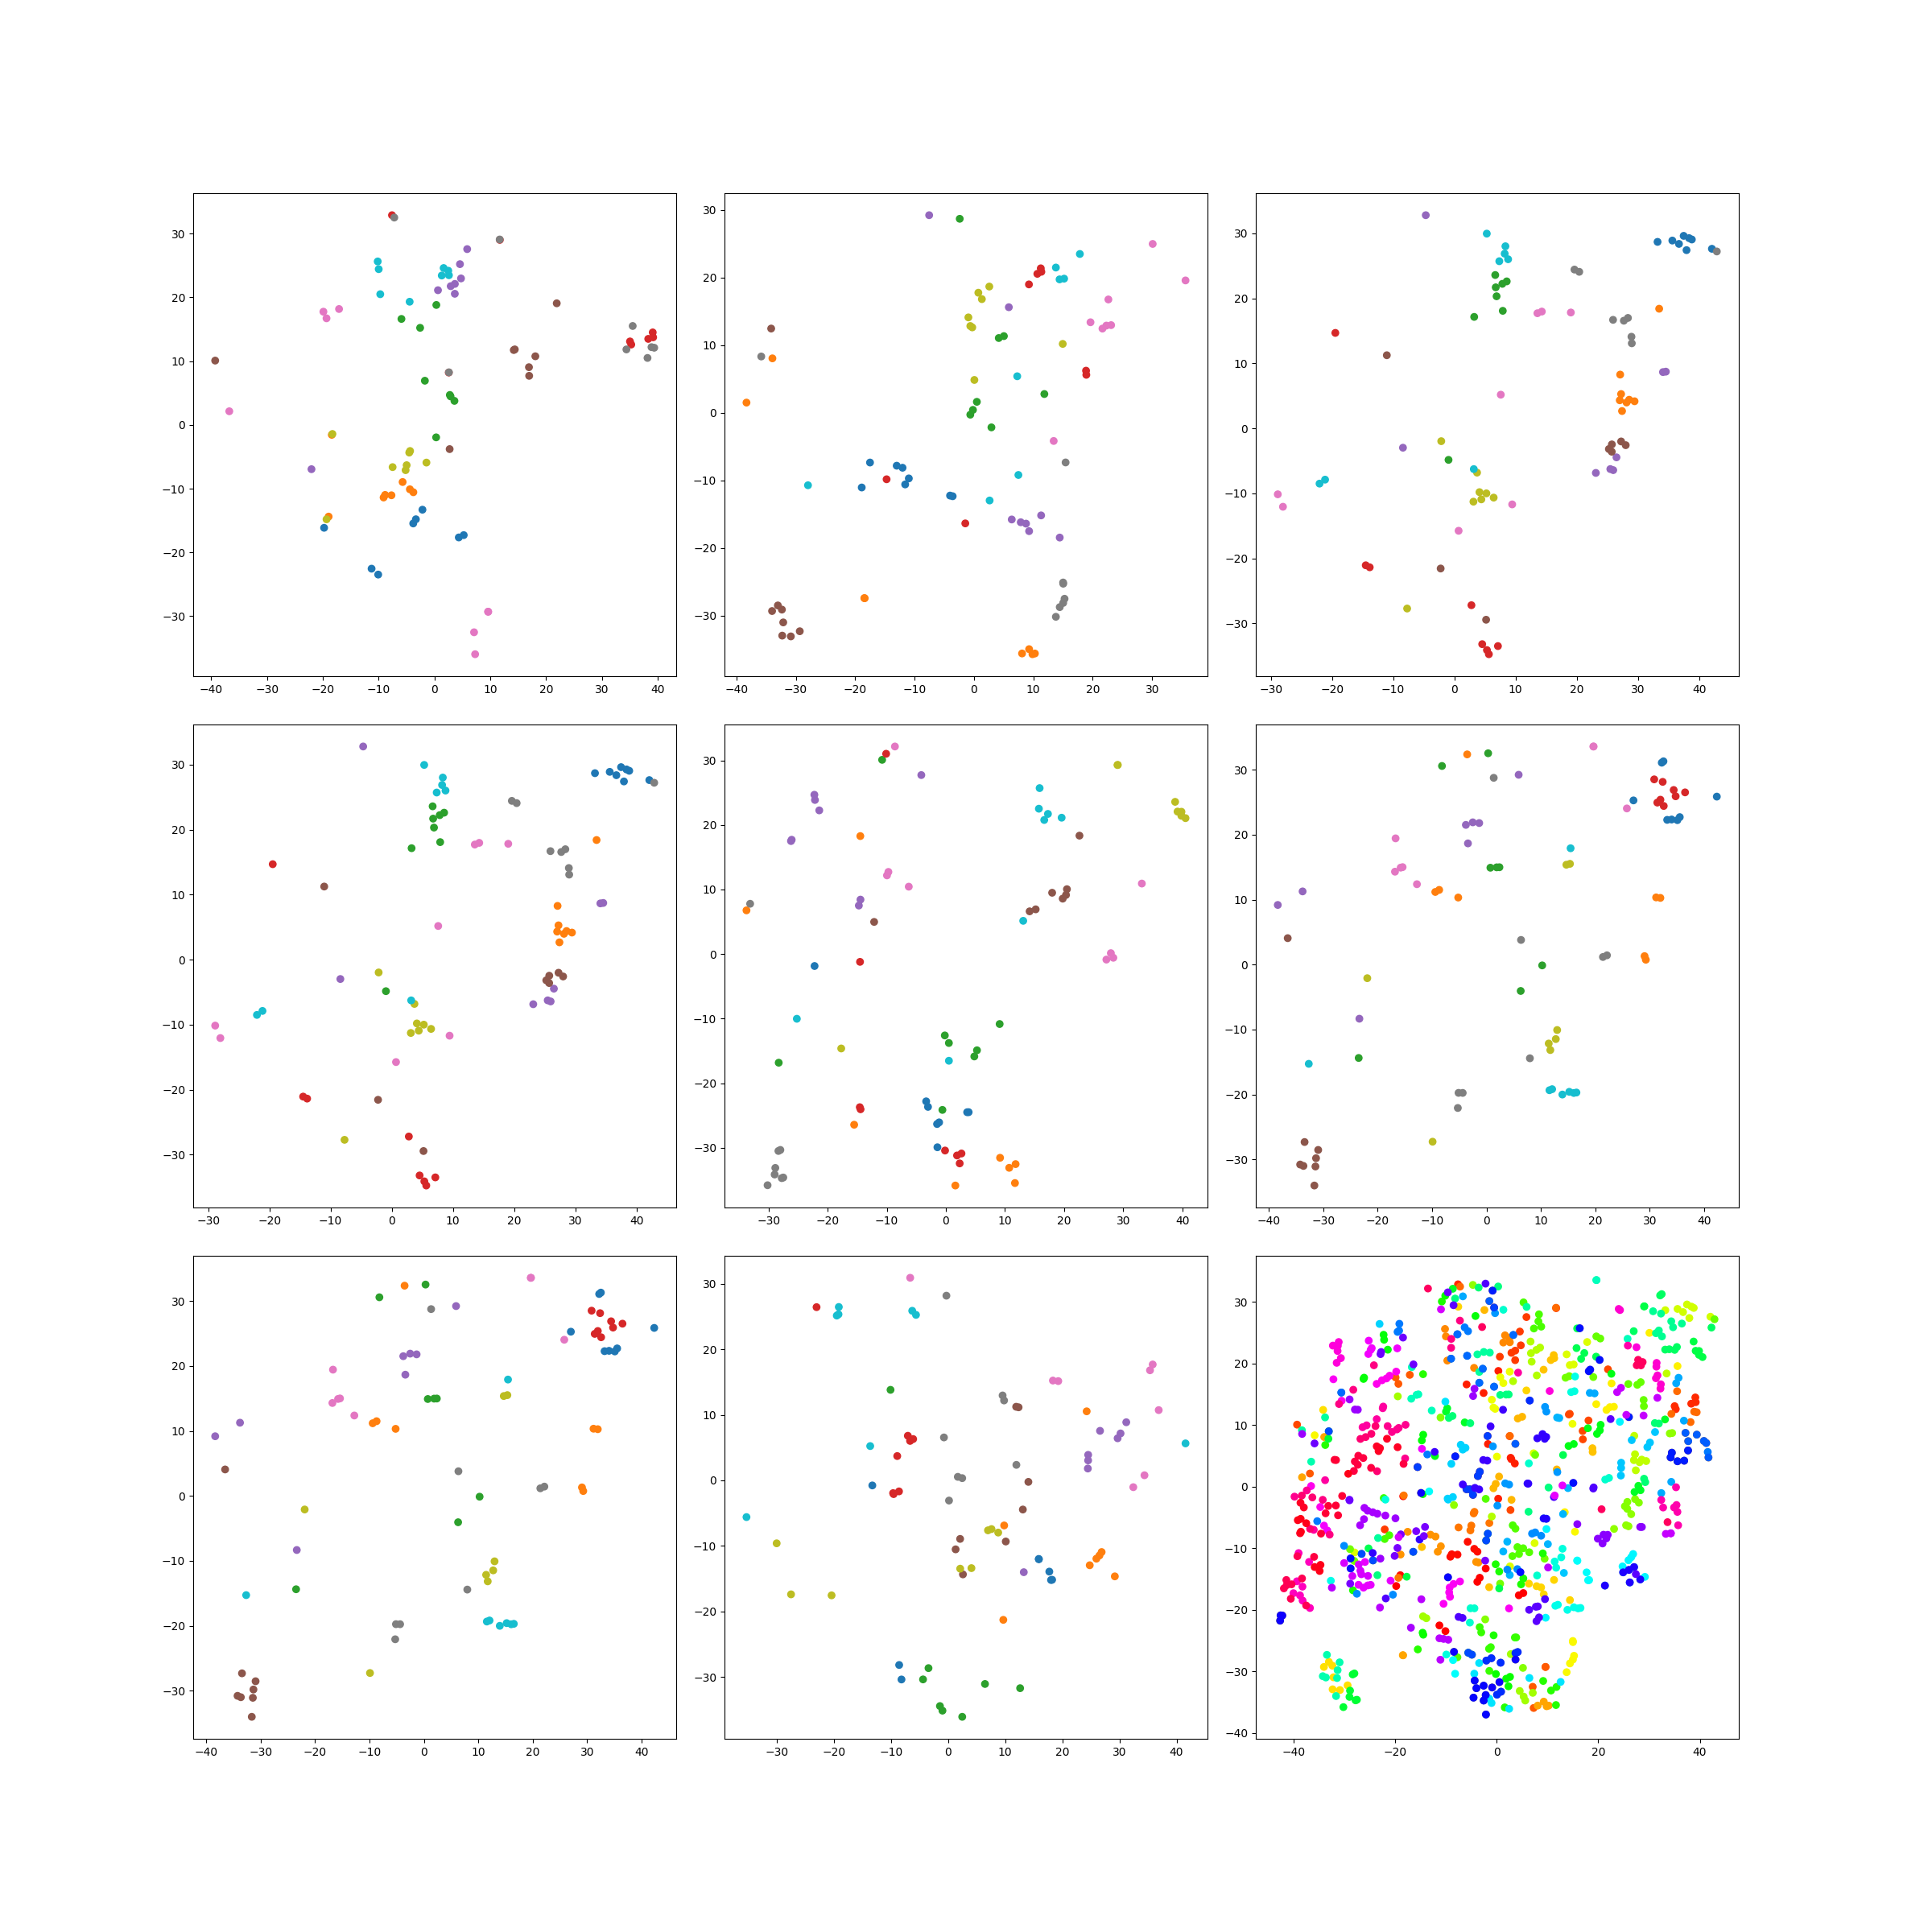
\includegraphics[scale=0.3]{./Chapter4/Figures/CLStsne_1}
\caption{First eight curve include graphs for 10 different subjects each, last curve shows separability of all 100 subjects.}
\label{fig:figure10}
\end{figure}

\subsection{VGG with triplet loss}
Now we used the triplet loss to train our VGG model. Triplet loss contains three different images namely anchor, positive and negative. Anchor and positive are from the same subject while the negative is different from our anchor. The triplet loss can be defined as in \ref{eq44}
\begin{equation}
	\begin{aligned}
		Loss = \sum^N_{i=1}[\vert\vert f^a_{i} - f^p_{i} \vert\vert^2_{2} - \vert\vert f^a_{i} - f^n_{i} \vert\vert^2_{2} + \alpha] 
\end{aligned}
\label{eq44}
\end{equation}

The figures for the L2 distance and t-sne are as shown in \ref{fig:figure11} and \ref{fig:figure12} respectively


\begin{figure}[htbp]
\centering
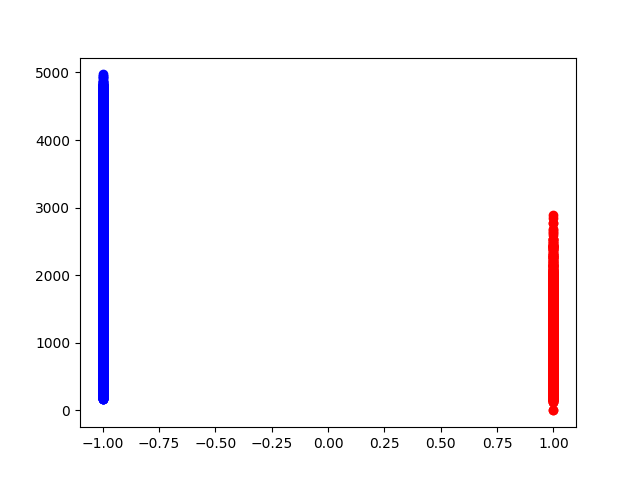
\includegraphics[scale=1]{./Chapter4/Figures/TRPnorms_pos_neg_1}
\caption{L2 distance for all positive and negative pairs. Here X = 1 stands for positive and X = -1 stands for negative pairs. Y axis represents the value of L2 distance}
\label{fig:figure11}
\end{figure}

\begin{figure}[htbp]
\centering
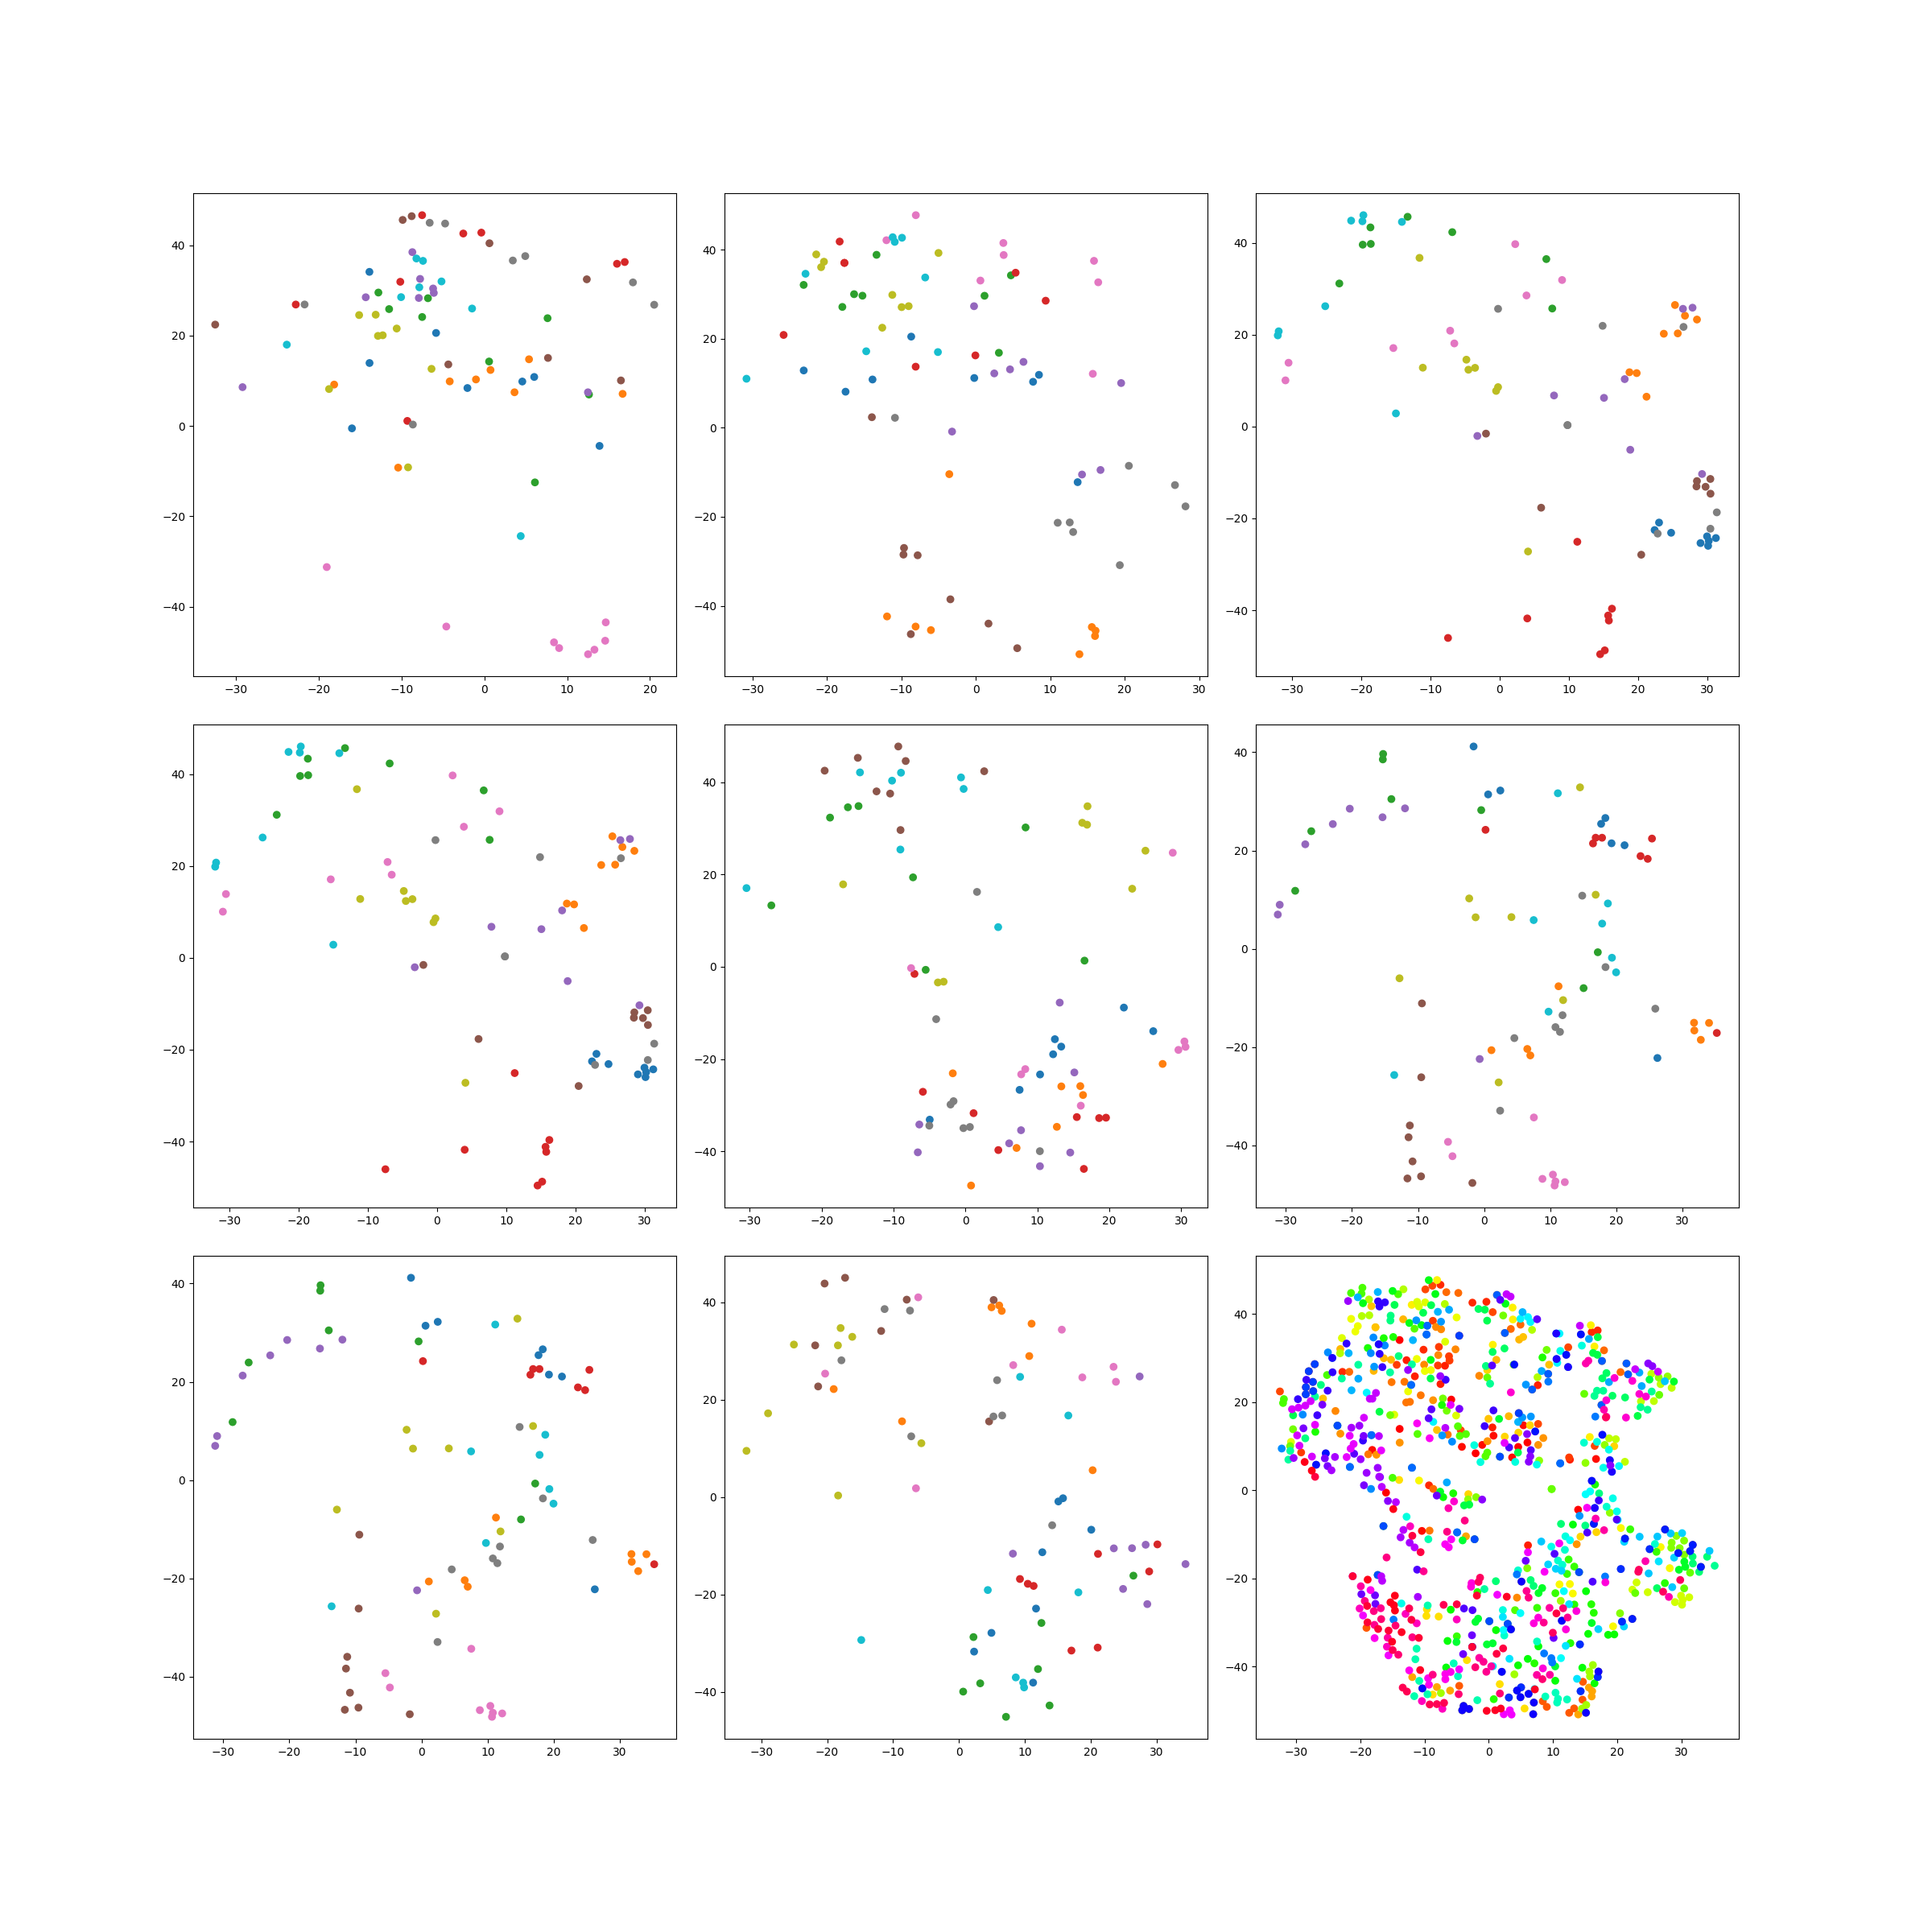
\includegraphics[scale=0.3]{./Chapter4/Figures/TRPtsne_1}
\caption{First seven curve include graphs for 10 different subjects each, last curve shows separability of all 100 subjects.}
\label{fig:figure12}
\end{figure}


Comparing all the above three methods we can say that triplet loss gives us better results as compared to others. The first two methods clearly are not capable of separating our dataset while the triplet loss has succeeded quite much (as compared to rest two).

Finally to increase the positive samples per subject we augmented our data to generate 10 different images subjecting to single image with different kinds of augmentation like Gaussian Blur, Affine, Crop, Emboss etc. Hence now our single subject contains images having 10 times larger than our previous samples and to reduce our network further we used squeezeNet \cite{Iandola2016SqueezeNetAA} instead of VGG16.

With the above modification, we trained our model on the FVC2002 dataset with augmentation and after 4-5 epochs we were able to generate unique hash codes of different subjects with an efficiency of 64 unique codes out of 100 subjects. We experimented keeping our anchor fixed for all the subjects in all the epochs. We were only changing the positive and negative samples of different subjects. Hence it is not guaranteed yet that the  hamming distance of the  generated hash codes of similar images will tend to zero, and will go further away from zero in case of negative samples.

